
\subparagraph{Calcolo della capacità di un condensatore con MATLAB}
Si ricorda il modello dell'elettrostatica
$$
\begin{cases}
\nabla \times \vec{E} = 0 &\text{in } \Omega \Rightarrow \vec{E} = -\nabla u\\
\nabla\cdot\vec{D} = 0 &\text{in }\Omega\text{ non ci sono cariche libere}\\
\vec{D} = \varepsilon\vec{E} &\text{in } \Omega\text{ materiale omogeneo ed isotropo}
\end{cases}
$$
Il modello si trasforma in questo caso nel problema dei valori al contorno
per l'equazione di Laplace con condizioni di Dirichlet sugli elettrodi
e condizione alla Neumann su una frontiera abbastanza lontana da approssimare
l'infinito.
$$
\begin{cases}
\nabla^2 u = 0 & \text{in } \Omega\\
\left.u\right|_{l_1} = V_1\\
\left.u\right|_{l_2} = 0\\
\left.\frac{\partial u}{\partial n}\right|_{\partial\Omega e} = 0
\end{cases}
$$
Le funzioni ``tenda'' solitamente utilizzate nei metodi agli elementi finiti
sono lineari a tratti, ad esempio la funzione $w_i$ vale $1$ nel nodo
in cui è valutata e decresce linearmente a $0$ nei nodi adiacenti.
Il grado del polinomio della funzione test può essere incrementato ma
si incrementano anche i problemi analitici dovuti al rispetto
delle condizioni al contorno e di raccordo, per questo motivo sono solitamente
utilizzati polinomi di grado 1.
\begin{figure}[H]
\centering
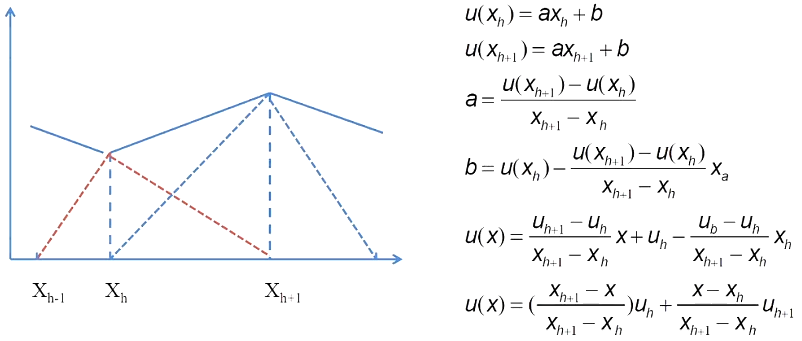
\includegraphics[width=0.7\linewidth]{funzione_tenda}
\caption{Espressione analitica funzione tenda di grado 1}
\end{figure}
Per ricostruire la funzione si esegue una combinazione lineare delle
funzioni tenda nei vari punti.

Per domini bidimensionali è ancora possibile eseguire una discretizzazione
in elementi triangolari, con funzioni lineari in due variabili,
la matrice dei coefficienti risultante è simmetrica e semidefinita
positiva, inoltre è una matrice sparsa, ossia i coefficienti pari a zero sono 
molto maggiori rispetto a quelli diversi da zero.
\begin{figure}[H]
\centering
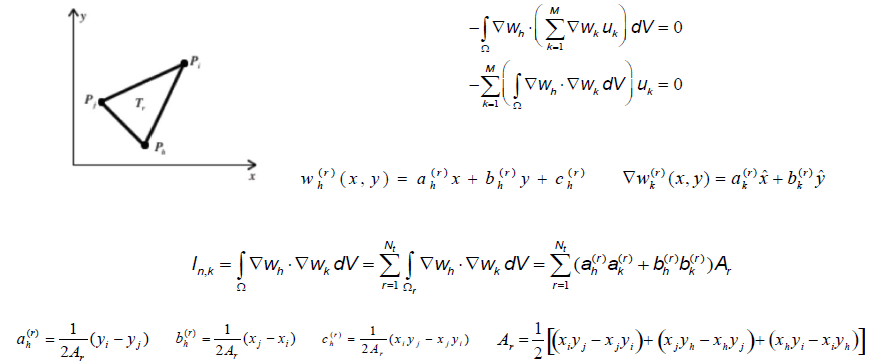
\includegraphics[width=0.7\linewidth]{tenda_bidimensionale}
\caption{Espressione funzione tenda bidimensionale}
\end{figure}





